\documentclass{ceurart}
\usepackage[show]{ed}
\usepackage{paralist}
\usepackage{amsmath}
\usepackage{cleveref}
\usepackage{listings}
\usepackage{tikz}
\usetikzlibrary{shapes.geometric} 
\usetikzlibrary{positioning}
\usetikzlibrary{arrows}
\usetikzlibrary{arrows.meta}

\lstset{
  basicstyle=\ttfamily,
}

\def\emph#1{\textbf{#1}}


% \title{Efficiently Linking Documents to Alignment Databases -- A Prototype-Based Exploration}
\title{Helping Humans Align Efficiently}

\author[1]{Jan Frederik Schaefer}
\author[2]{Michael Kohlhase}

\conference{Workshop on Math Datasets: alignments and comparisons (ALIGN2025),
  October 10, 2025, Brasilia, Brazil}

\begin{document}
\maketitle
Both formal and informal mathematical knowledge is fragmented across many different systems and formats.
Aligning the concepts across these resources
is a key contribution towards making the data FAIR
(Findable, Accessible, Interoperable, Reusable).
% A first step towards combining these resources
% and making the data FAIR (Findable, Accessible, Interoperable, Reusable)
% is aligning their concepts.
An alignment, for us, links a concept from one system to a concept in another system,
indicating that they represent the same object or idea.
We ignore the added complexity that concepts may only be similar,
but not a precise match (see \cite{10.1007/978-3-319-62075-6_7}
for a discussion of this issue).
Most authors and curators try to generate alignments from existing datasets
automatically (via rule-based matching, machine learning, or LLM techniques),
but few parallel corpora exist for mathematics, and unsupervised approaches
seem difficult for the subtle distinctions crucial in mathematical knowledge.
We claim that human-created alignments are necessary
-- to ensure high quality, or at least to create datasets
for training and evaluation.

\paragraph{Example}
Alignments can be created between diverse resources,
including knowledge graphs, libraries for automated theorem provers,
and documents.
As a running example, consider the simple sentence
% and encounter the sentence
\begin{quote}
Let $n$ be a natural number.
\end{quote}
where we want to align the concept reference ``natural number'' with
the corresponding WikiData concept.
Such an alignment could, for example,
provide additional information to the reader,
or determine the prerequisite knowledge for understanding the document.
It could also be a first step towards full formalization:
if we also align e.g.\ the type of natural numbers
in Lean's mathlib with Wikidata,
we have an indirect alignment between the document and mathlib.

% Creating such alignments is difficult.
In our example there are, in fact, three possible alignment targets:
\begin{compactitem}
\item \texttt{Q21199} (natural numbers, possibly including 0)
\item \texttt{Q28920044} (positive integers, i.e.\ natural numbers excluding 0)
\item \texttt{Q28920052} (non-negative integers, i.e.\ natural numbers including 0)
\end{compactitem}
This kind of ambiguity is a major challenge for automated alignment.
While a human aligner, especially one familiar with the document,
may well be able to correctly disambiguate,
they face the additional challenge of remembering what concepts exist
or searching for them, which takes significant time and effort.

% For a human aligner,
% there is the additional challenge of knowing which concepts exist


% We claim that machine learning techniques are not yet capable of
% making the right choice sufficiently reliably,
% which puts the burden of creating alignments on humans.
% Even if machine learning techniques are successful,
% we will need human aligners for a gold standard and
% possibly for training data.

\paragraph{Contribution}
In this paper,
we propose a workflow for human alignment supported by a simple tool
that iterates over the data to be aligned
and presents the user with a list of alignment candidates to select from
(see \Cref{fig:workflow}).
% we will outline how the alignment workflow can
% be made much more efficient with if (relatively simple) tools
% suggest alignment candidates that the user can select from.
For the implementation, we build on the snify architecture for selection-based,
corpus-based semantic annotation~\cite{KohSch:safc25}
and extend it, prototypically, to the alignment problem.

\begin{figure}
    \centering
    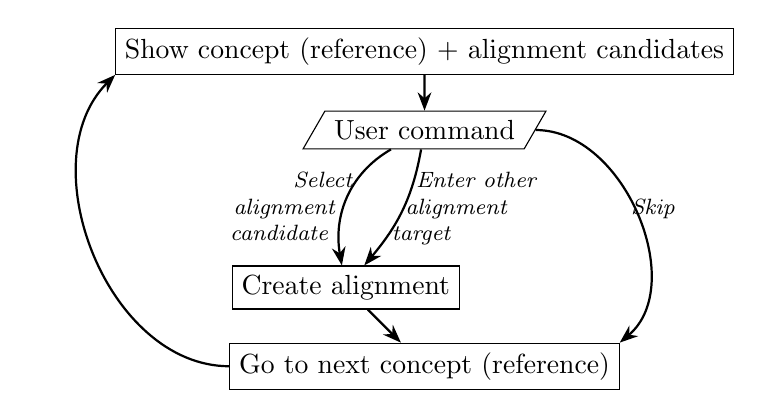
\begin{tikzpicture}
        \node[draw,rectangle] (show) at (0, 2) {Show concept (reference) + alignment candidates};
        \node[trapezium left angle=60, trapezium right angle=-60,trapezium,draw] (command) at (0, 1) {User command};
        \node[draw,rectangle] (create) at (-1, -1) {Create alignment};
        \draw[-Stealth,thick] (command) to[in=100,out=210] (create);
        \draw[-Stealth,thick] (command) to[in=50,out=260] (create);
        \node at (-1.65, 0) {\itshape\footnotesize\begin{tabular}rSelect\;\ \\alignment\quad\ \\candidate\quad\;\ \end{tabular}};
        \node at (0.5, 0) {\itshape\footnotesize\begin{tabular}l\quad Enter other\\\;\;alignment\\target\end{tabular}};
        \node[draw,rectangle] (next) at (0, -2) {Go to next concept (reference)};
        \draw[-Stealth,thick] (show) -- (command);
        \draw[-Stealth,thick] (create) -- (next);
        \draw[-Stealth,thick] (command) to[out=0,in=40] (next.north east);
        \node at (2.9, 0) {\itshape\footnotesize Skip};
        \draw[-Stealth,thick] (next) to[out=180,in=225] (show.south west);
    \end{tikzpicture}
    \caption{Flowchart of tool support for human aligners.}\label{fig:workflow}
\end{figure}



% and present a extension of the snify tool~\cite{KohSch:safc25}
% that implements this workflow.


\begin{figure}
    \centering
    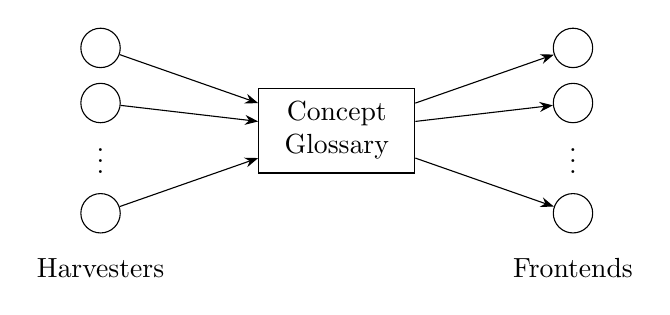
\begin{tikzpicture}[xscale=3, yscale=0.7]
        \node[circle,draw,minimum size=0.5cm] (h1) at (-1, 1.5) {};
        \node[circle,draw,minimum size=0.5cm] (h2) at (-1, 0.5) {};
        \node at (-1, -0.4) {$\vdots$};
        \node[circle,draw,minimum size=0.5cm] (h3) at (-1, -1.5) {};
        \node at (-1, -2.5) {Harvesters};
        \node[draw, rectangle] (catalog) at (0, 0) {\begin{tabular}cConcept\\Glossary\end{tabular}};
        \node[circle,draw,minimum size=0.5cm] (f1) at (1, 1.5) {};
        \node[circle,draw,minimum size=0.5cm] (f2) at (1, 0.5) {};
        \node at (1, -0.4) {$\vdots$};
        \node[circle,draw,minimum size=0.5cm] (f3) at (1, -1.5) {};
        \node at (1, -2.5) {Frontends};
        \draw[-Stealth] (h1) -- (catalog);
        \draw[-Stealth] (h2) -- (catalog);
        \draw[-Stealth] (h3) -- (catalog);
        \draw[-Stealth] (catalog) -- (f1);
        \draw[-Stealth] (catalog) -- (f2);
        \draw[-Stealth] (catalog) -- (f3);
    \end{tikzpicture}
    \caption{
        Proposed architecture:
        Custom harvesters extract a concept glossary from concept collections.
        The concept glossary can be used by frontends customized
        to the data we want to align.
    }\label{fig:architecture}
\end{figure}



\paragraph{Proposed Architecture}
To support the workflow from \Cref{fig:workflow},
we propose an architecture centered around a \emph{concept glossary}
(see \Cref{fig:architecture}).
The concept glossary is extracted from the concept collection
that we want to align with -- in our example, WikiData --
using a custom \emph{harvester}. % -- for example, using a SPARQL query.
The concept glossary contains for each concept
a unique \emph{identifier}, a human-readable \emph{description},
and a set of \emph{verbalizations} (natural language renderings of the concept).
For example, a concept glossary extracted from WikiData could have the following entry:
\begin{compactitem}
\item \textit{identifier}: \texttt{https://www.wikidata.org/wiki/Q28920044}
\item \textit{description}: ``\textit{positive integer} (integer greater than zero; natural number explicitly excluding zero)``
\item \textit{verbalizations}: ``positive integer'', ``integer greater than zero'', ``natural number'', \textellipsis
\end{compactitem}
The description is necessary to help the user identify the correct concept
as the identifiers are not human-readable.
The (language-specific) verbalizations can be used to find alignment candidates.
In practice, not every concept collection has verbalizations,
but alignments can mitigate this:
if concept $A$ is aligned with concept $B$ and $B$ has the verbalization $v$,
then we can also use $v$ as a verbalization for $A$.

The concept glossary is used by \emph{frontends} that enable
the alignment workflow sketched in \Cref{fig:workflow}.
The details depend on what we want to align:
aligning phrases in a document is, for example,
very different from aligning concepts in an ontology.
Note that harvesters and frontends are largely independent
as they are only connected via the concept glossary.
This facilitates reusing harvesters for new frontends
or, vice versa, reusing frontends for harvesters
for new different concept collections.





% The concept glossary is used b
% 
% 
% Note that the alignment catalog is independent of the source collection.
% While an alignment support tool requires significant customization
% for the source collection (aligning phrases in a document is
% very different from aligning concepts in an ontology),
% it can easily support different catalogs.

% Concretely, we focus on the workflow where a (human) aligner iterates over
% concepts or concept references in a \emph{source collection}
% to align them, where possible,
% with concepts from a \emph{target collection}.
% While we require that the target collection has unique concept identifiers
% -- for easy referencing --
% this is not necessary for the source collection.
% For example, we can align text fragments in a document
% by annotating them with an identifier from the target collection.




% Without dedicated tool support,
% the author has to either recall the correct alignment target from
% memory or search for it, and then edit the document to add the alignment annotation.
% The workflow is much more efficient, if a tool
% presents the user with a list of alignment candidates
% (like the three options above),
% from which the user can select the correct one.
% 
% To make this work, the target collection has to provide
% an \emph{alignment catalog},
% which links each concept identifier to a human-readable description
% and a set of \emph{verbalizations} (natural language renderings of the concept).

\paragraph{Building on snify}
The snify tool~\cite{KohSch:safc25} implements
a a workflow similar to the one shown in \Cref{fig:workflow}
for semantic annotation.
Both the harvester and the frontend act on \LaTeX\ documents
that use the \texttt{stex} package for semantic markup.
Using the snify tool has significantly increased
the efficiency of annotators, especially for novices who
are not deeply familiar with the domain model (i.e.\ who
do not know the identifiers by heart).

In this paper, we build on the snify architecture
to support alignment outside of the sTeX ecosystem.
Concretely, we have added a harvester for mathematical concepts from WikiData,
rudimentary support for aligning formulae,
a frontend for aligning HTML documents,
and a browser-based user interface,
which helps with the annotation of HTML documents.

% The sTeX ecosystem, which uses diverse semantic markup to drive
% learning support systems,
% faced a similar challenge, which was recently addressed by the snify system\cite{KohSch:safc25}.
% In this paper, we present a prototypical extension of the snify system
% for efficient alignment that is independent of the sTeX ecosystem.
% Concretely, we have added the option to use WikiData as the concept database,
% rudimentary support for annotating formulae,
% the ability to annotate HTML documents,
% and a browser-based user interface, which
% helps with the annotation of HTML documents.

The snify tool is implemented as a command line application.
It steps through the phrases in a document that match verbalizations
from the concept glossary
and presents the user with a list of potential targets.
To recognize inflected forms -- e.g.\ ``continuities'' instead of ``continuity''
-- snify uses an off-the-shelf stemmer.
\Cref{fig:snify} shows the tool in action.
The user can select the correct entry from the list by entering its number,
which then creates the alignment by inserting a macro into the document
(here e.g.\ \lstinline.\wdalign{Q28920044}{natural number}).
If the user does not want to create an alignment,
there are many other commands to skip phrases,
undo annotations, modify the selection, etc.

% This workflow transforms the problem from a \emph{recollection}
% problem, where the user has to remember the correct alignment target
% or otherwise spend time searching for it,
% to a \emph{selection} problem, where the user can
% pick the correct option from a list of candidates.
% In the sTeX ecosystem, the snify tool has significantly increased
% the efficiency of annotators, especially for novices who
% are not deeply familiar with the domain model (i.e.\ the concept database).


\begin{figure}
    \centering
    \includegraphics[width=0.7\textwidth]{img1.png}
    \caption{Screenshot of aligning
    \LaTeX\ documents with WikiData concepts using snify.}\label{fig:snify}
\end{figure}

% In the background, snify uses a verbalization catalog
% that links concept, here WikiData identifiers,
% to their natural language renderings (verbalizations).
% WikiData has both language-specific labels and synonyms.
% For example, \lstinline.Q28920044. has the
% label ``positive integer'' and lists ``natural number''
% as a synonym.
% This verbalization catalog drives the search for potential targets
% and the selection of candidates.
% To recognize inflected forms -- e.g.\ ``continuities'' instead of ``continuity''
% -- snify uses an off-the-shelf stemmer.

\paragraph{Supporting Formulae and HTML}
Aside from verbalizations,
WikiData also has formula notations
for many concepts, including \LaTeX\ notations like \lstinline.\mathbb{N}.
(in the concept glossary, we could treat them as verbalizations in another language).
This allows us to use the same workflow to align formula fragments,
but there are significant limitations:
operators can be aligned, but their arguments are not marked, and
some operators, like the invisible multiplication in ``$ax$'',
are not represented by a glyph at all.
In sTeX, the solution is essentially to write down
a semantic representation of the formula and generate the presentation from it.
A grammar-based approach to generate the semantic representation
for ``conventional'' \LaTeX\ formulae
in collaboration with a human annotator was presented in~\cite{VreWelKam:tsmmdui24}.
For alignments, this approach could be considered too invasive.

% There is no reason to restrict the approach to \LaTeX\ documents.
To explore other formats, we have added support for HTML documents,
where the alignments are stored in HTML attributes.
Reading plain HTML in the command line interface is not ideal,
especially for complex MathML formulae.
To improve this, we have created a browser-based interface
that closely imitates the command line interface
but can render HTML instead of showing the raw source (see \cref{fig:snify-browser}).

\begin{figure}
    \centering
    \includegraphics[width=0.7\textwidth]{img2.png}
    \caption{Screenshot of the browser-based snify interface.
    Here, a MathML operator is being annotated.
    }\label{fig:snify-browser}
\end{figure}

\paragraph{Conclusion}
In summary, we have described a workflow for efficient human alignment
based on an concept glossary
and presented a prototypical implementation based on the snify tool
that explores this workflow
for the alignment of text and formulae in \LaTeX\ and HTML documents
with WikiData concepts.
% 
% In summary, we have demonstrated that the snify approach for sTeX annotation
% can generalize to alignments with other concept databases
% and document formats.
While the formula alignment is rather limited,
it was relatively easy to implement and could be improved in the future.
On a higher level, this shows how relatively simple and naive tools
can enable much more efficient alignment workflows,
and we hope to inspire the community to think about other tools
that could help alignment authors.
% -- be it text-to-database or database-to-database alignment.

% \printbibliography

\bibliography{references}


% Document-to-database alignments are just annotations of specific
% text fragments or formula fragments in the document.
% For example, the text fragment ``natural number'' could be
% with the WikiData concept for natural numbers (Q21199).
% % For formulas, the annotation target can be less clear, for example because
% % some operations, such as the multiplication in ``$ax$'',
% % may not be represented by a glyph.
% % Depending on the document format, there there may still be
% % be an (invisible) symbol that can be annotated -- e.g.\ the unicode character for invisible multiplication.
% % An alternative is to annotate the whole sub-expression, i.e.\ the operation
% % including the operands.\ednote{these remarks break the flow}
% 
% Annotations can be created manually, e.g.\ by the authors,
% or automatically using machine learning techniques.
% Here, we focus on high-quality manual annotation,
% claiming that machine learning models are not sufficiently
% reliable, especially in research-level documents where training data is necessarily scarce.
% Presenting a user with wrong but convincing alignments
% is arguably worse than not providing any alignments at all.
% 
% The key challenge is to convice authors to actually create alignment annotations,
% as it is additional effort with little immediate benefit.
% To change the balance, we could either increase the benefit
% by providing better services based on the annotations,
% or reduce the effort by providing better annotation tools.
% Here we focus on the latter.
% 
% There is already an ecosystem of annotation tools, annotation formats
% and services based on them, developed in the KWARC group:
% \begin{compactitem}
% \item Annotation formats for \LaTeX (sTeX), HTML (FTML),
%     and, prototypically, Microsoft Word (WOIDE).
% \item Services for education (the ALeA platform)
% \item Tool support for manual annotation in sTeX
%     (snify and the sTeX IDE) and, prototypically, in Word (WOIDE).
% \end{compactitem}
% While there have been significant efforts to allow gradual adoption
% and remain as flexible as possible,
% potential users ultimately have to commit to a relatively
% complex ecosystem system of actively developed research software.
% As such, a dedicated teacher may be willing to invest time to
% move their teaching materials into this ecosystem
% to get the benefits of the ALeA learning platform,
% but a researcher writing a paper likely will not.
% 
% In this paper, we present a prototypical extension of the snify system
% for light-weight alignment independent of this ecosystem.
% The snify tool has been developed for the efficient annotation of natural language text
% with concept references and has been used to create an estimated 10,000 annotations.
% 
% Figure\ednote{TODO} shows
% 
% % Example:
% % Let $n < m$ be natural numbers.
% 
% 
% 
% % However, we can adapt some of the ideas and tools
% % for lightweight alignment of documents.
% % For example, the snify system has been designed
% % for large-scale manual creation of sTeX annotations.
% % By adapting it for alignment, we can
% % take advantage of
% 
% 
% % The focus of this paper is the alignment
% % of concept references in documents -- e.g.\ scientific papers -- with a concept database.
% % We will use WikiData as the concept database in our examples.
% % As WikiData is often referenced in other alignment databases,
% % e.g.\ MathGloss~\cite{mathgloss:arxiv},
% % this would also provide indirect alignments with other systems.
% % 
% % These document-to-database alignments are just annotations of specific
% % text fragments or formula fragments in the document.
% % For example, the text fragment ``natural number'' could be
% % with the WikiData concept for natural numbers (Q21199).
% % For formulas, the annotation target can be less clear, for example because
% % some operations, such as the multiplication in ``$ax$'',
% % are not represented by a glyph.
% % Depending on the document format, there there may still be
% % be an (invisible) symbol that can be annotated -- e.g.\ the unicode character for invisible multiplication.
% % An alternative is to annotate the whole sub-expression, i.e.\ the operation
% % including the operands.\ednote{these remarks break the flow}
% % 
% % Annotations can be created manually, e.g.\ by the authors,
% % or automatically using machine learning techniques.
% % Here, we focus on high-quality manual annotation,
% % claiming that machine learning models are not sufficiently
% % reliable, especially in research-level documents where training data is necessarily scarce.
% % Presenting a user with wrong but convincing alignments
% % is arguably worse than not providing any alignments at all.
% % 
% % The key challenge is to convice authors to actually create alignment annotations,
% % as it is additional effort with little immediate benefit.
% % To change the balance, we could either increase the benefit
% % by providing better services based on the annotations,
% % or reduce the effort by providing better annotation tools.
% % Here we focus on the latter.
% % 
% % There is already an ecosystem of annotation tools, annotation formats
% % and services based on them, developed in the KWARC group:
% % \begin{compactitem}
% % \item Annotation formats for \LaTeX (sTeX), HTML (FTML),
% %     and, prototypically, Microsoft Word (WOIDE).
% % \item Services for education (the ALeA platform)
% % \item Tool support for manual annotation in sTeX
% %     (snify and the sTeX IDE) and, prototypically, in Word (WOIDE).
% % \end{compactitem}
% % While there have been significant efforts to allow gradual adoption
% % and remain as flexible as possible,
% % potential users ultimately have to commit to a relatively
% % complex ecosystem system of actively developed research software.
% % As such, a dedicated teacher may be willing to invest time to
% % move their teaching materials into this ecosystem
% % to get the benefits of the ALeA learning platform,
% % but a researcher writing a paper will likely not.
% % 
% % However, we can adapt some of the ideas and tools
% % for lightweight alignment of documents.
% % For example, the snify system has been designed
% % for large-scale manual creation of sTeX annotations.
% % By adapting it for alignment, we can
% % take advantage of
% 

\end{document}
